% Presentation Beamer
% Characteristics:
% -- Several Themes
% -- 

%%%%%%%%%%%%%%%%%%%%%%
%%%%%%%%%%%%%%%%%%%%%%
%%% Document Start %%%
%%%%%%%%%%%%%%%%%%%%%%
%%%%%%%%%%%%%%%%%%%%%%

\documentclass{beamer}

%%%%%%%%%%%%%%%%%%%%%%%%
%%% General Settings %%%
%%%%%%%%%%%%%%%%%%%%%%%%

%%% Packages %%%
\usepackage{verbatim}
\usepackage{graphicx}
\usepackage{subfig}
\usepackage{float}
\usepackage[ruled,linesnumbered]{algorithm2e}

%%% Definitions %%%

%%% Theme Selection %%%
%\usetheme{AnnArbor}
\usetheme{Antibes}
%\usetheme{Bergen}
%\usetheme{Berkeley}
%\usetheme{Berlin}
%\usetheme{Boadilla}
%\usetheme{boxes}
%\usetheme{CambridgeUS}
%\usetheme{Copenhagen}
%\usetheme{Darmstadt}
%\usetheme{default}
%\usetheme{Frankfurt}
%\usetheme{Goettingen}
%\usetheme{Hannover}
%\usetheme{Ilmenau}
%\usetheme{JuanLesPins}
%\usetheme{Luebeck}
%\usetheme{Madrid}
%\usetheme{Malmoe}
%\usetheme{Marburg}
%\usetheme{Montpellier}
%\usetheme{PaloAlto}
%\usetheme{Pittsburgh}
%\usetheme{Rochester}
%\usetheme{Singapore}
%\usetheme{Szeged}
%\usetheme{Warsaw}

%%% PDF Subject Catalog %%%
% - This is only inserted into the PDF information catalog. Can be left
% out.
\subject{Reinforcement Learning}

%%% Institution Logo %%% - Optional
% If you have a file called "university-logo-filename.xxx", where xxx
% is a graphic format that can be processed by latex or pdflatex,
% resp., then you can add a logo as follows:
\pgfdeclareimage[height=0.5cm]{university-logo}{university-logo-filename}
\logo{\pgfuseimage{university-logo}}

%%%%%%%%%%%%%%%%%%%%%%%%%%
%%% Presentation Cover %%%
%%%%%%%%%%%%%%%%%%%%%%%%%%

%%% Presentation Title %%%
\title{Defenses against Adversarial Examples}

%%% Subtitle %%% - Optional
%\subtitle{and Other RL Methods}

%%% Presentation Authors %%%%
% - Give the names in the same order as the appear in the paper.
% - Use the \inst{?} command only if the authors have different
%   affiliation.
\author{Keller Jordan$^1$, Rene Gutierrez$^2$, Brett G\"ohre$^3$}

%%% Author Affiliation %%% - Optional
% - Use the \inst command only if there are several affiliations.
% - Keep it simple, no one is interested in your street address.
\institute[University of California Santa Cruz]
{
\inst{1}%
Department of Computer Science \\
UCSC
\and
\inst{2}%
Department of Applied Mathematics \& Statistics \\
UCSC
\and
\inst{3}%
Department of Physical \& Biological Sciences \\
UCSC
}


%%% Conference Name and Information %%% - Optional
% - Either use conference name or its abbreviation.
% - Not really informative to the audience, more for people (including
%   yourself) who are reading the slides on-line
\date{CMPS290, Winter 2018}

%%% Table of Contents %%% - Optional
% Delete this, if you do not want the table of contents to pop up at
% the beginning of each subsection:
\begin{comment}
\AtBeginSubsection[]
{
\begin{frame}<beamer>{Outline}
\tableofcontents[currentsection,currentsubsection]
\end{frame}
}
\end{comment}

%%%%%%%%%%%%%%%%%%%%%%%%%%%%
%%% Presentation Content %%%
%%%%%%%%%%%%%%%%%%%%%%%%%%%%

\begin{document}
	
	%%% Title Page %%%
	\begin{frame}
		\titlepage
	\end{frame}
	
	
	%%% Outline %%% - Optional
	% - You might wish to add the option [pausesections]
	% - Section and subsections will appear in the presentation overview
	% and table of contents.
	%\begin{frame}{Outline}
	%  \tableofcontents
	%\end{frame}
	
	%%% Body %%%
	\graphicspath{{figures/}}


		\section*{Introduction}
	
	\begin{frame}{Motivation}
		\begin{block}{Neural Networks at risk of being fooled}
			\begin{itemize}
				\item Types of attacks:
				\begin{itemize}
					\item White box– Access to Neural Network model and weight configuration
					\item Black box– Only know the task of targeted Neural Network, archictecture and current weights unknown
				\end{itemize}
				\item Alarming strategy:
				\begin{itemize}
					\item Learn attacks on white box model trained on similar data to black box target
					\item Attacks on white box carry over to black box, especially when ensembled (ref. Bo Li's slides)
				\end{itemize}
			\end{itemize}
		\end{block}
	\end{frame}
	
	\begin{frame}{Motivation}
		\begin{block}{Attempts at defending}
			\begin{itemize}
				\item Only good until attacker learns about them (ref. Bo Li's slides)
				\item Motivates attempt to use random preprocessing of input images
				\item Does being more data-efficient make attacks harder? CapsNet?
				\item Reflecting on reconstructed image from adversarial image could be sign of being fooled
			\end{itemize}
		\end{block}
	\end{frame}
	
	\begin{frame}{Random Projection Matrix}
		\begin{block}{Key Idea}
			Using a Random Projection Matrix unknown to the Attacker to modify the attack perturbation to defend against it.
		\end{block}
	\end{frame}
	
	
	\begin{frame}{Detection of Adversarial Examples using Reconstruction Error}
		\begin{block}{Key Idea}
			The training loss function is augmented with L2 distance between original image and a reconstruction from the final output of a capsule network. The capsule network output is useful here since it outputs a vector that has more information about the input than a single scalar quantifying the existence of the class.
		\end{block}
	\end{frame}
	
	\begin{frame}{Multi-task training as Defense}
		\begin{block}{Key Idea}
			MNIST and FashionMNIST have very different low-level features. Does joint training on FashionMNIST act as a regularizor that strengthens the MNIST classification against attacks? (Results will be featured in write-up).
		\end{block}
	\end{frame}
	
	\section*{Random Projection Matrices}
	
	\begin{frame}{Idea}
		\begin{block}{}
			\begin{itemize}
				\item Some Black-Box Adversarial Attacks rely on adding noise-like small perturbations $ \epsilon $  to an Input $ x $.
				\item Can we transform the noise into a less powerful attack using a Random Projection Matrix $ \Phi $ unknown to the attacker. That is, can we go from:
				$$ x + \epsilon \to \Phi x + \Phi \epsilon $$
				\item Does $ \Phi \epsilon $ retains it's attacking power?
			\end{itemize}
		\end{block}
	\end{frame}
	
	\begin{frame}{Method}
		\begin{block}{}
			\begin{itemize}
				\item We worked on the MNIST data set.
				\item We generated 2 sets of Adversarial Attacks based on 2 different architectures, Logistic Regression and Convolutional Neural Networks.
				\item In order to generate the Attacks, we added noise-like small perturbations using a trained network and then optimizing for misclassification, while trying to reduce the size of the perturbation.
			\end{itemize}
		\end{block}
	\end{frame}
	
	\begin{frame}{Method}
		\begin{block}{}
			\begin{itemize}
				\item The first set was created of a Logistic Regression architecture, consisting in the best attacks using as inputs the tests sets, obtaining 758 such attacks.
				\item The second set was similarly created on a CNN trained to achieve 95\% accuracy on the validation set, obtaining 440 attacks.
				\item We tested 2 strategies, one Compression Matrix (from 784 to 196) and one Expansion Matrix (from 784 to 1960).
			\end{itemize}
		\end{block}
	\end{frame}
	
	\begin{frame}{Methods}
		\begin{figure}[h!]
			\centering
			\caption{\enspace Examples of the Adversarial Attacks created under the 2 Architectures. The left side shows the attacks created with the Logistic Regression, while the right side was created using a CNN.}
			\subfloat[Adversarial Attack for 3]{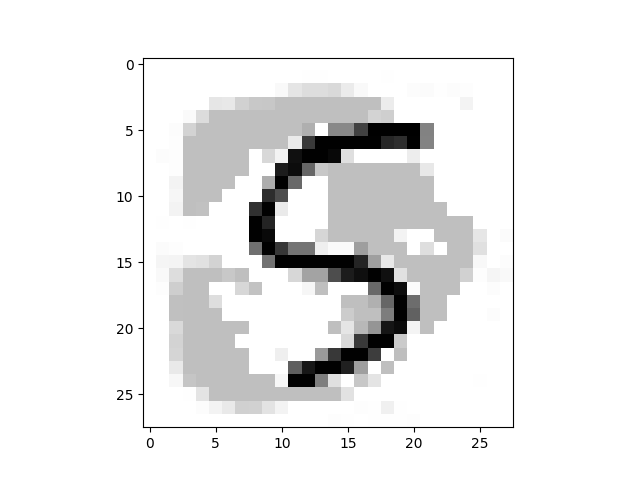
\includegraphics[width=0.25\linewidth]{advImg.png}} 
			\subfloat[Noise  ]{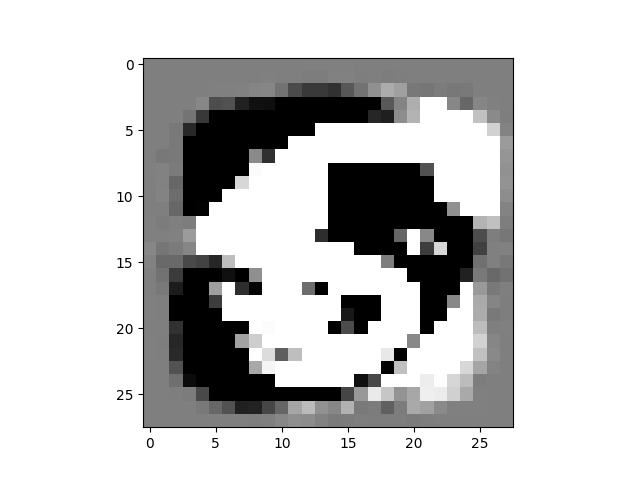
\includegraphics[width=0.25\linewidth]{advNoi.png}}  
			\subfloat[Adversarial Attack for 3]{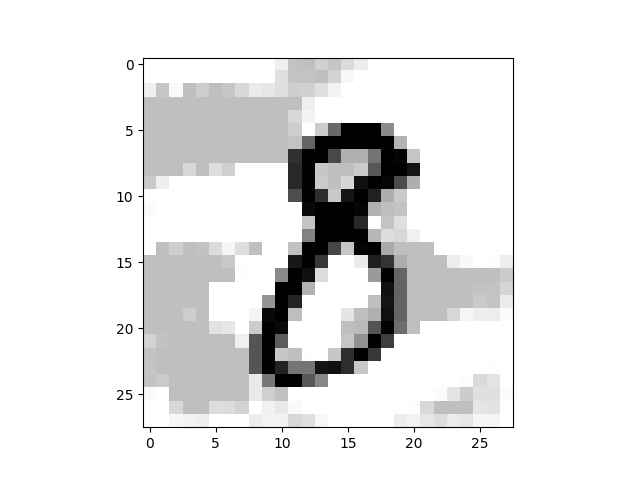
\includegraphics[width=0.25\linewidth]{advImgCnn.png}} 
			\subfloat[Noise  ]{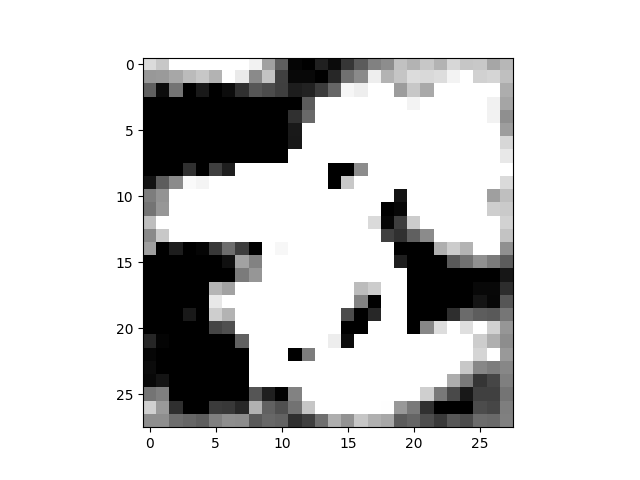
\includegraphics[width=0.25\linewidth]{advNoiCnn.png}} 
		\end{figure}
	\end{frame}
	
	\begin{frame}{Results}
		\begin{table}
			\caption{\enspace Accuracy for the 5 different methods, using the test set and the adversarial examples generated by Logistic Regression and CNN architectures.}
			\label{tab1}
			\begin{tabular*}{\hsize}{@{\extracolsep{\fill}}cccc}
				\hline
				\\[-7pt]
				\multicolumn{1}{c}{\it Method}                    & 
				\multicolumn{1}{c}{\it Test Set}                  & 
				\multicolumn{1}{c}{\it Log Adversarial} & 
				\multicolumn{1}{c}{\it CNN Adversarial}      \\
				\hline
				\\[-5pt]
				Logistic Reg             & 92.00\% & 0.00\%  & 3.41\%  \\
				CNN 90\%                 & 89.82\% & 8.71\%  & 5.23\%  \\
				CNN 95\%                 & 94.64\% & 9.50\%  & 9.50\%  \\
				CNN 99\%                 & 98.63\% & 60.95\% & 11.36\% \\
				Com Log 196  dim         & 89.56\% & 0.00\%  & 5.00\%  \\
				Exp Log 1960 dim         & 91.07\% & 0.00\%  & 3.64\% 
			\end{tabular*}
		\end{table}
	\end{frame}
	
	\begin{frame}{Results}
		\begin{figure}[h!]
			\centering
			\caption{\enspace Confusion Matrices for the True Target and Predicted Target for the Compression Matrix and Examples generated with the Logistic Regression architecture.}
			\subfloat[Confusion Matrix for True Class]{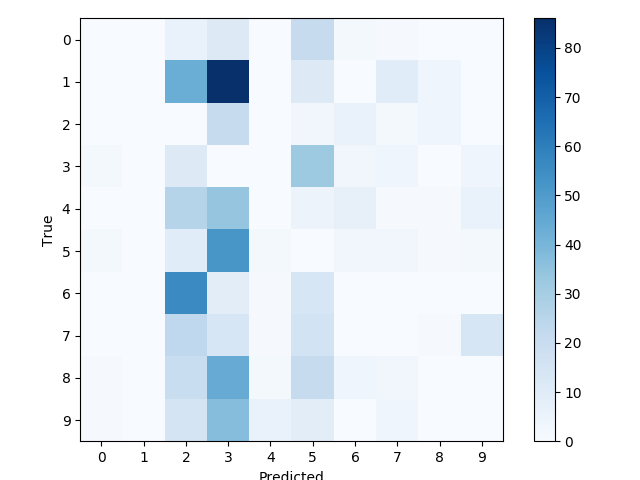
\includegraphics[width=0.5\linewidth]{confussionMatrixAdvTrueCom.png}} 
			\subfloat[Confusion Matrix for Target Class]{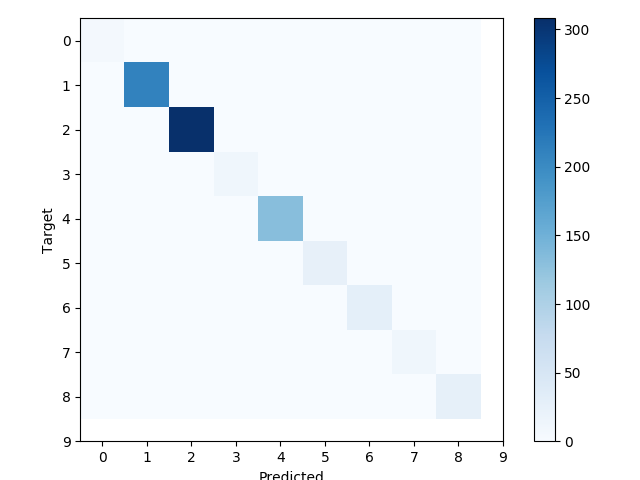
\includegraphics[width=0.5\linewidth]{confussionMatrixAdvTarCom.png}}   \\
		\end{figure}
	\end{frame}
	
	\begin{frame}{Results}
		\begin{figure}[h!]
			\centering
			\caption{\enspace Confusion Matrices for the True Target and Predicted Target for the Expansion Matrix and Examples generated with the Logistic Regression architecture.}
			\subfloat[Confusion Matrix for True Class]{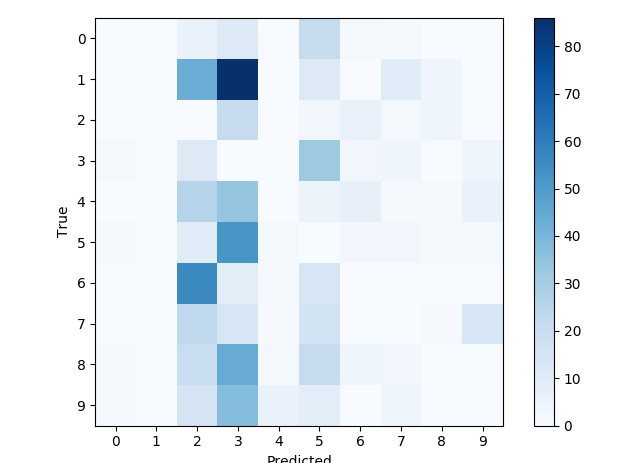
\includegraphics[width=0.5\linewidth]{confussionMatrixAdvTrueExp.png}} 
			\subfloat[Confusion Matrix for Target Class]{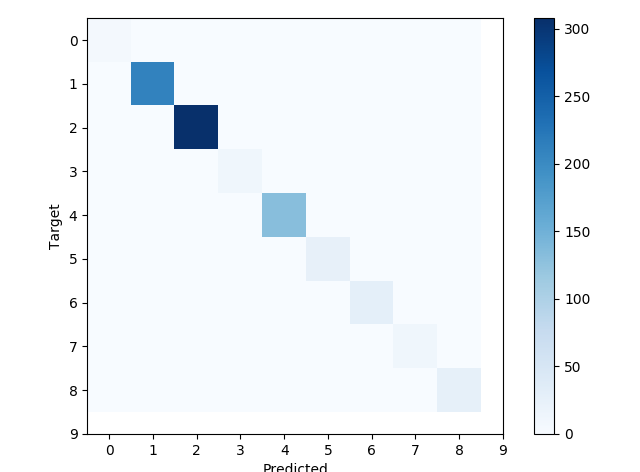
\includegraphics[width=0.5\linewidth]{confussionMatrixAdvTarExp.png}}   \\
		\end{figure}
	\end{frame}
	
	\begin{frame}{Results}
		\begin{figure}[h!]
			\centering
			\caption{\enspace Weights for 2, for the Compression, Expansion and Regular Logistic Regression.}
			\subfloat[Compression]{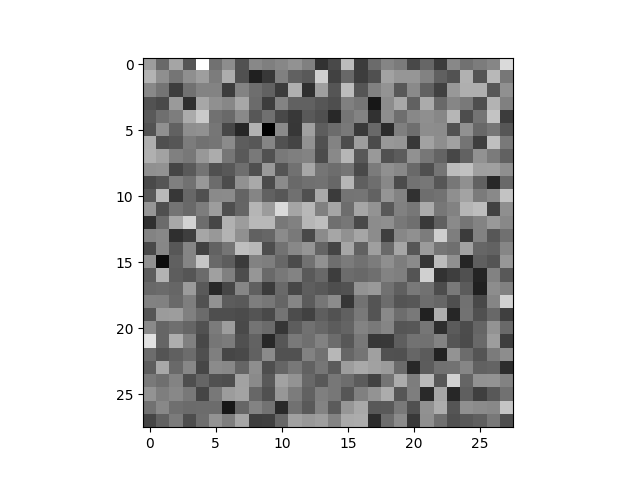
\includegraphics[width=0.33\linewidth]{com2.png}}
			\subfloat[Expansion]{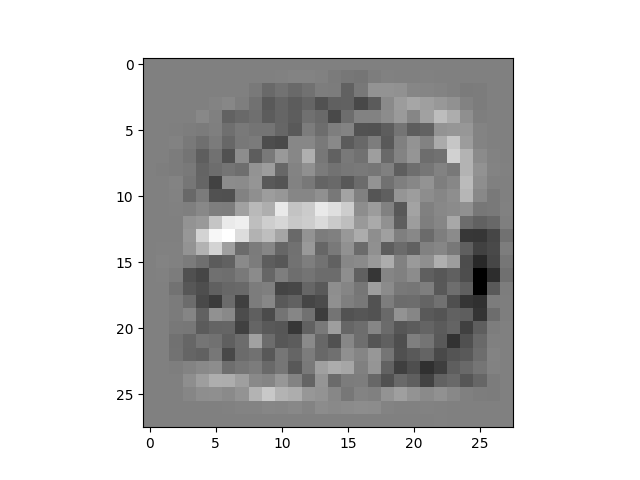
\includegraphics[width=0.33\linewidth]{exp2.png}}
			\subfloat[Regular]{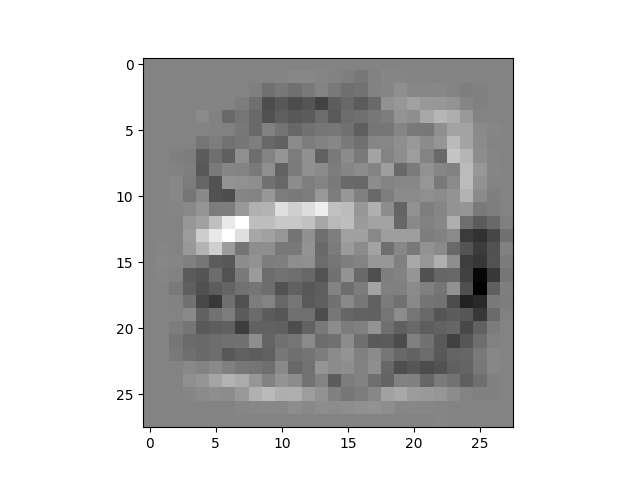
\includegraphics[width=0.33\linewidth]{reg2.png}}  
		\end{figure}
	\end{frame}
	
	\begin{frame}{Results}
		\begin{figure}[h!]
			\centering
			\caption{\enspace Weights for 2, for the Compression t0 196, Compression to 392, Compression to 588 and Regular Logistic Regression.}
			\subfloat[196]{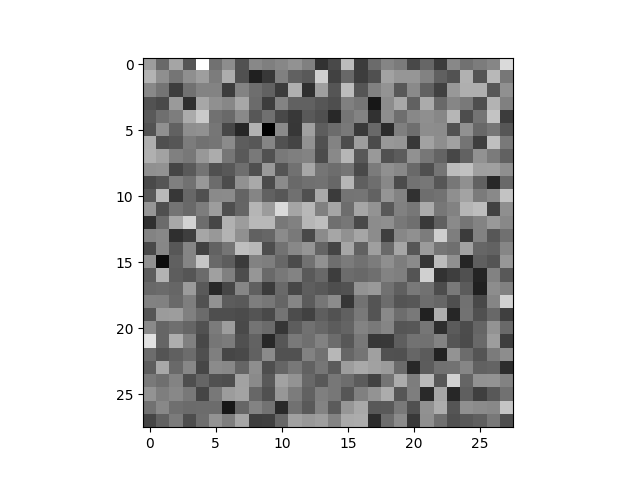
\includegraphics[width=0.25\linewidth]{com2.png}}
			\subfloat[392]{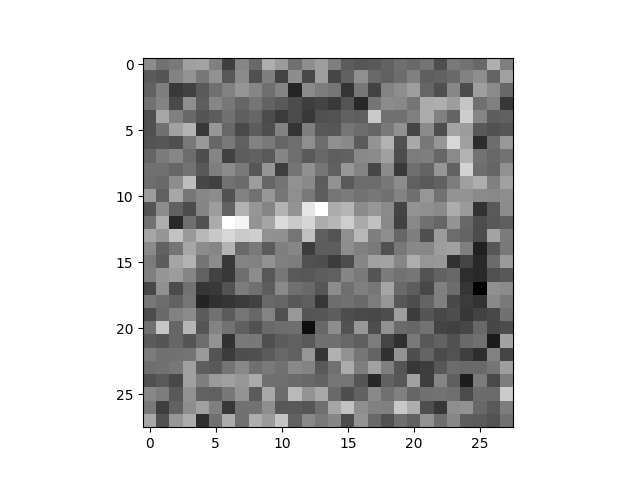
\includegraphics[width=0.25\linewidth]{co22.png}}
			\subfloat[588]{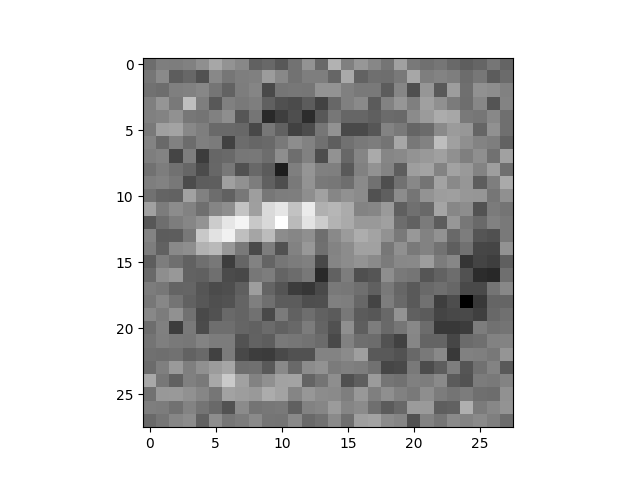
\includegraphics[width=0.25\linewidth]{co32.png}}
			\subfloat[Reg]{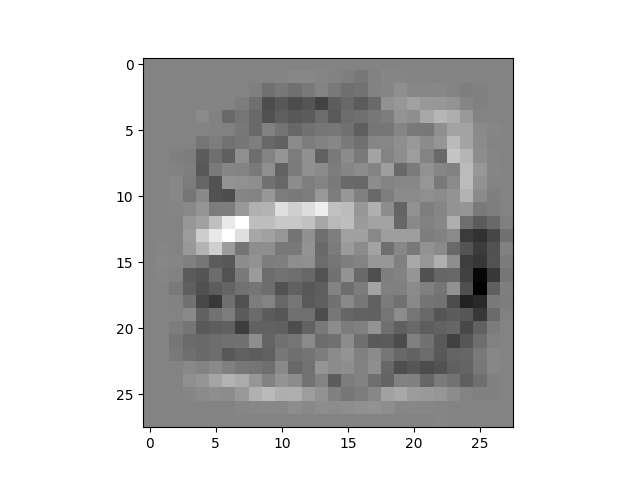
\includegraphics[width=0.25\linewidth]{reg2.png}}  
		\end{figure}
	\end{frame}
	
	\begin{frame}{Multi-task training as Defense}
		\begin{block}{Key Idea}
			We explore the robustness outcome of joint training on FashionMNIST while training an MNIST classifier. This multi-task network will be attacked by a white box attacks effective on neural net trained only on MNIST. MNIST and FashionMNIST have very different features, so we expect the results to be different from merely obtaining white box attacks on subsets of MNIST and applying them to full MNIST. (Results to be featured in write-up).
		\end{block}
	\end{frame}
	
	\section*{Optimizer Robustness}
	
	\begin{frame}{Optimizer Robustness}
		\begin{block}{Optimizers Studied}
			\begin{center}
				\begin{tabular}{ l | l | l }
					Method & SGD & EG \\ \hline
					Rule & 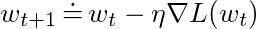
\includegraphics[width=4cm]{sgd_rule} & 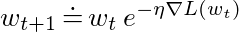
\includegraphics[width=4cm]{eg_rule}
				\end{tabular}
			\end{center}
		\end{block}
		\begin{itemize}
			\item Used extension of EG to +/- weights case for training
		\end{itemize}
	\end{frame}
	
	\begin{frame}{Procedure}
		\begin{itemize}
			\item Train FC 784-100-10 using GD and EG$\pm$ on MNIST
			\item Run untargeted adversarial attack methods
			\begin{itemize}
				\item Gradient Ascent
				\item Iterative Fast Gradient Sign
			\end{itemize}
			\item Compare resulting models and adversarial examples
			\begin{itemize}
				\item Number of iters to fool
				\item Transferability of strong attacks
				\item Average perturbation
			\end{itemize}
		\end{itemize}
	\end{frame}
	
	\begin{frame}{Examples}
		\centering
		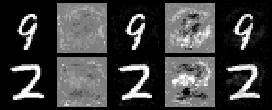
\includegraphics[width=\textwidth]{mnist_attacks}
	\end{frame}
	
	\begin{frame}{Attack Difficulty}
		\begin{block}{Number of iterations to fool network}
			\begin{center}
				\begin{tabular}{ l | l | l }
					Method / Optimizer & SGD & EG \\ \hline
					Gradient Ascent & $60.9 (\pm 32.3)$ & $85.1 (\pm 40.5)$ \\ \hline
					Iterative Fast Gradient Sign & $52.0 (\pm 26.1)$ & $91.0 (\pm 43.5)$
				\end{tabular}
			\end{center}
		\end{block}
		\begin{itemize}
			\item A network is defined as ``fooled" when its prediction changes
		\end{itemize}
	\end{frame}
	
	\begin{frame}{Average Perturbation}
		\centering
		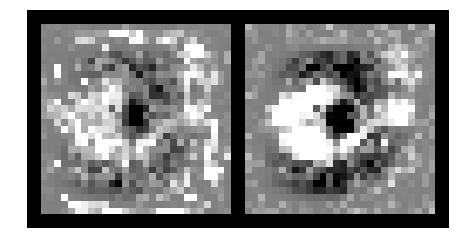
\includegraphics[width=\textwidth]{avg_attack_3}
		
		SGD (left), EG$\pm$ (right)
	\end{frame}
	
	\begin{frame}{Transferability Results}
		\begin{block}{Probability of success on other optimizer}
			\begin{center}
				\begin{tabular}{ l | l | l }
					Method / Src$\rightarrow$Dst & SGD$\rightarrow$EG & EG$\rightarrow$SGD  \\ \hline
					Gradient Ascent & 67.4\% & 99.0\% \\ \hline
					Iterative Fast Gradient Sign & 88.2\% & 99.8\%
				\end{tabular}
			\end{center}
		\end{block}
		\begin{itemize}
			\item Iterations held constant at 200 (should be comparably strong)
		\end{itemize}
	\end{frame}
	
	\begin{frame}{Results}
		\begin{itemize}
			\item Requires 1.5$\times$ stronger attacks to fool EG-trained model
			\item EG shows some robustness to attacks transferred from SGD
			\item SGD is not robust to attacks transferred to EG
			\item Attacks against EG make more sense w.r.t. expected structure of digit space
		\end{itemize}
	\end{frame}

	\section*{Reconstruction as a Defense}
	
	\begin{frame}{Defending using Reconstruction Error}
		\begin{block}{Basic idea}
			\begin{itemize}
				\item Use an architecture that reconstructs input images (CapsNet)
				\item Model will reconstruct some element of decoder-space for fooled class
				\item Adversarial images are unlikely to be in this space
				\item Expect high reconstruction error (MSE)
			\end{itemize}
		\end{block}
	\end{frame}
	
	\begin{frame}{Capsule Network Refresher}
		\centering
		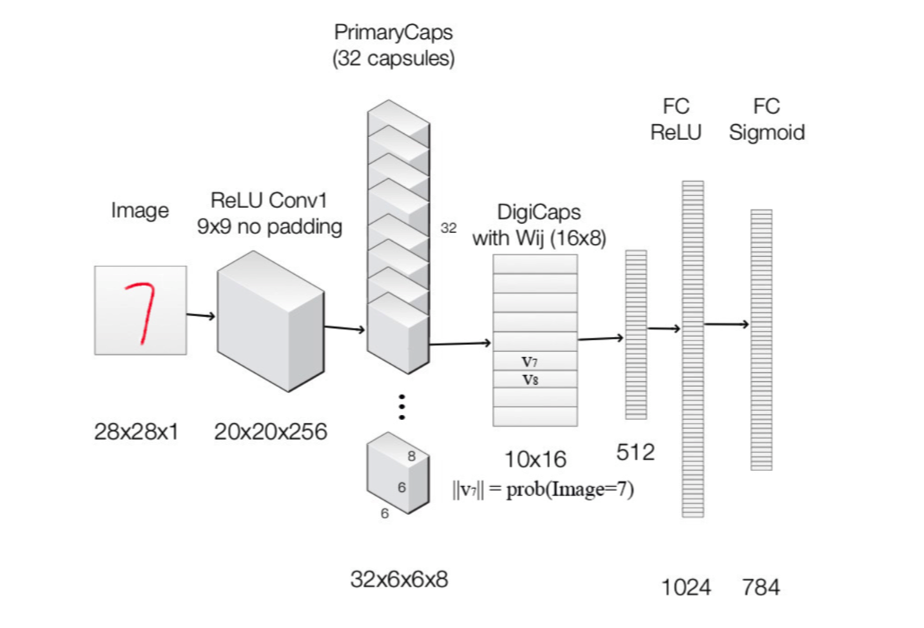
\includegraphics[width=\textwidth]{caps_recon}
	\end{frame}
	
	\begin{frame}{Reconstructions}
		\centering
		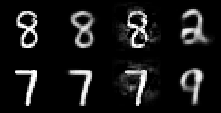
\includegraphics[width=\textwidth]{recon-fig5}
	\end{frame}
	
	\begin{frame}{Reconstructions}
		\centering
		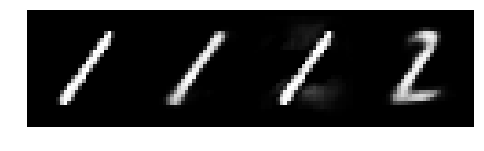
\includegraphics[width=\textwidth]{recon-fig4}		
		
		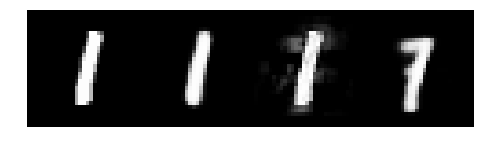
\includegraphics[width=\textwidth]{recon-fig3}
	\end{frame}
	
	\begin{frame}{Results}
		\centering
		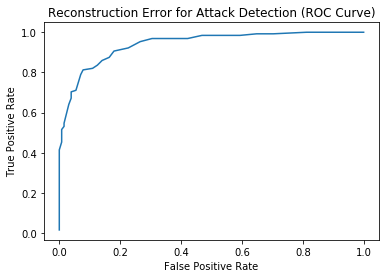
\includegraphics[width=10cm]{mse_roc}
	\end{frame}
	
	\begin{frame}{Results}
		\begin{itemize}
			\item Method successfully detects $\sim$70\% of of attacks with 5\% false-positive rate
			\item Could be improved by better loss function
			\item Unknown vulnerability to white-box attacks
			\item Expect good black-box performance due to variability of decoders and loss functions
		\end{itemize}
	\end{frame}
	
	
	% All of the following is optional and typically not needed.
	\begin{comment}
	\appendix
	\section<presentation>*{\appendixname}
	\subsection<presentation>*{For Further Reading}
	
	\begin{frame}[allowframebreaks]
	\frametitle<presentation>{For Further Reading}
	
	\begin{thebibliography}{10}
	
	\beamertemplatebookbibitems
	% Start with overview books.
	
	\bibitem{Author1990}
	A.~Author.
	\newblock {\em Handbook of Everything}.
	\newblock Some Press, 1990.
	
	
	\beamertemplatearticlebibitems
	% Followed by interesting articles. Keep the list short. 
	
	\bibitem{Someone2000}
	S.~Someone.
	\newblock On this and that.
	\newblock {\em Journal of This and That}, 2(1):50--100,
	2000.
	\end{thebibliography}
	
	\end{frame}
	
	\begin{itemize}
	\item
	Outlook
	\begin{itemize}
	\item
	Something you haven't solved.
	\item
	Something else you haven't solved.
	\end{itemize}
	\end{itemize}
	
	\end{comment}
	
\end{document}